\documentclass{article}
\usepackage{icmc,amsmath}
\usepackage{graphicx}
\usepackage{url}

\title{Freedom in TAPESTREA! Voice-Aware Track Manipulations}

\threeauthors
  {Tom Lieber} {Princeton University \\ lieber@princeton.edu}
  {Ananya Misra} {Princeton University \\ amisra@cs.princeton.edu}
  {Perry Cook} {Princeton University \\ prc@cs.princeton.edu}

% LyX command for teletype
\newcommand{\noun}[1]{\textsc{#1}}

\begin{document}

\maketitle

\begin{abstract}
Tracks in TAPESTREA have too long been oppressed, unable to choose which other
tracks they hang out with, and only able to be modified in fixed groups. They
had no say in their own lives, no individuality. That ends today. We advocate
\noun{Freedom} in TAPESTREA by way of VTAPS, where every track can be
interacted with as a distinct, \noun{Free} entity. Only thus can it contribute
fully to the larger sound scene. Please sponsor our movement by downloading
TAPESTREA at \\
{\tt \small http://taps.cs.princeton.edu/}.

TAPESTREA is environmental audio editing software that encourages the user to
work with pitched sounds in terms of salient frequencies that modulate over
time, otherwise called tracks. While TAPESTREA has provided the means for
manipulating these tracks as groups (called ``templates''), the aim of this
project -- VTAPS -- is to allow the user to manipulate tracks individually or
in arbitrary groups.  This allows for advanced manipulations to be performed
quickly and with more control than when templates were indivisible units. It
inspires and enables features for manipulating the audio in ways that are
useful for voice recordings and musical instruments.

% This needs mention of voice manipulation
% Blah, blah, voice, blah, blah, other instruments as well. zoink
\end{abstract}

\section{Introduction}

TAPESTREA \cite{recompose} is a framework for creating music by re-composing 
existing sounds. It lets users extract desired portions of a recording, 
and stores them as {\it sound templates} of different types based on the modeling 
technique best suited for the selection. TAPESTREA supports the three-step 
workflow of extracting reusable sound templates from selected time-frequency 
regions in a recording, transforming these templates independently, and 
re-synthesizing the transformed templates to create new music.

The types of templates extracted can roughly correspond to foreground and 
background components of an audio recording. {\it Stochastic background} is the 
ambient noise that characterizes the background ``din'' of an environment. 
{\it Transient events} are brief, noisy, non-pitched audio events like door slams or 
claps. {\it Sinusoidal events} correspond to stable sinusoidal components of a sound. 
Voices, bird chirps, and other components perceived as pitched foreground events work 
well as sinusoidal events. 

Typically, a sinusoidal event template in TAPESTREA can be interactively extracted and later transformed 
as a single unit. The current work, VTAPS, facilitates more in-depth manipulation of sinusoidal templates. VTAPS adds a user interface area (or ``face''\footnote{TAPESTREA's interface is
imagined to be spread across the faces of a cube, where each face is a
different screen and caters to a different step of the editing process.}) that allows the user to 
interact with the building blocks of sinusoidal templates, tracks. In particular, VTAPS adds 
track-level manipulations relevant for voice processing. In this paper, we  
discuss the place of tracks in TAPESTREA, how they are interacted with by the user and 
internally by the software, and some applications of the new track selection and 
modification functionality. 


%TAPESTREA is a system that encourages the three-step workflow of extraction of
%audio's components, transformation of those components' parameters, and
%resynthesis into new soundscapes.  Rather than work with audio at the sample
%level, TAPESTREA works with sound data as combinations of these sinusoidal,
%transient, and stochastic components, called templates. Transient noises are
%non-pitched audio like door slams or claps, and stochastic noise is the random
%ambient noise that characterizes the ``din'' of an environment. This research
%focused primarily on sinusoidal templates, and information on transient and
%stochastic templates can be found in [3][4][5][6][7][8]...

%The user interface area (called a ``face'' \footnote{TAPESTREA's interface is
%imagined to be spread across the faces of a cube, where each face is a
%different screen and caters to a different step of the editing process.}) that
%VTAPS adds to TAPESTREA allows the user to interact with the building blocks of
%sinusoidal templates, tracks. In this paper, we first discuss the place of
%tracks in TAPESTREA, how they are interacted with by the user and internally by
%the software, then some of the uses of the added track selection/modification
%functionality.


\section{Related Work}
% Make this section much bigger and move to beginning
% Serra, Fitts, Lemur, MQ, etc

%SPEAR (Sinusoidal Partial Editing Analysis and Resynthesis) is a related
%software application by Michael Klingbeil \cite{spear}. It is essentially what
%the group face would be like were it its own application rather than an
%extension of TAPESTREA. It supports selection of tracks (``partials'') from a
%spectrogram-like display similar to that in the group face, immediate playback
%of the selected partials, and various tools for modifying tracks like frequency
%shifting, frequency transposition, time translation.

TAPESTREA makes use of the Spectral Modeling Synthesis (SMS) paradigm \cite{sms}, which 
in turn extends the original sinusoidal modeling algorithm \cite{mq} by introducing 
the concept of ``sines plus noise''. SMS depends on the idea that some parts of a sound suit 
a sinusoidal model, while others are closer to spectrally shaped noise. It  
originally modeled musical instrument sounds, but TAPES\-TREA applies it to arbitrary sounds 
at the user's discretion. 

Related existing software includes the CLAM library \cite{clam}, Lemur \cite{lemur}, and AudioSculpt \cite{audiosculpt}, which allow high-level sinusoidal analysis, transformation, and re-synthesis. 
However, they lack the interactive parametric control over all stages of processing offered by 
TAPESTREA. Another difference is that TAPESTREA allows the use of the ChucK \cite{chuck} 
programming language for precise scripting, which is especially powerful on re-synthesis. 

Another related software tool is SPEAR \cite{spear}, which supports the selection of sinusoidal 
tracks (partials) from a graphical interface, immediate playback of the selected partials, 
and various track modifications such as frequency shifting and transposition, and time 
translation. This perhaps comes closest to the VTAPS interface. However, VTAPS is specially 
designed to modify sinusoidal templates within TAPESTREA. These modified templates 
can then be used in conjunction with stochastic background, transients, and other templates 
to create a rich piece of music or sound design. Further, TAPESTREA offers certain track-level manipulations not offered by SPEAR, including some short-cuts geared towards voice processing. 

\section{Track Editing in TAPESTREA}

\begin{figure}
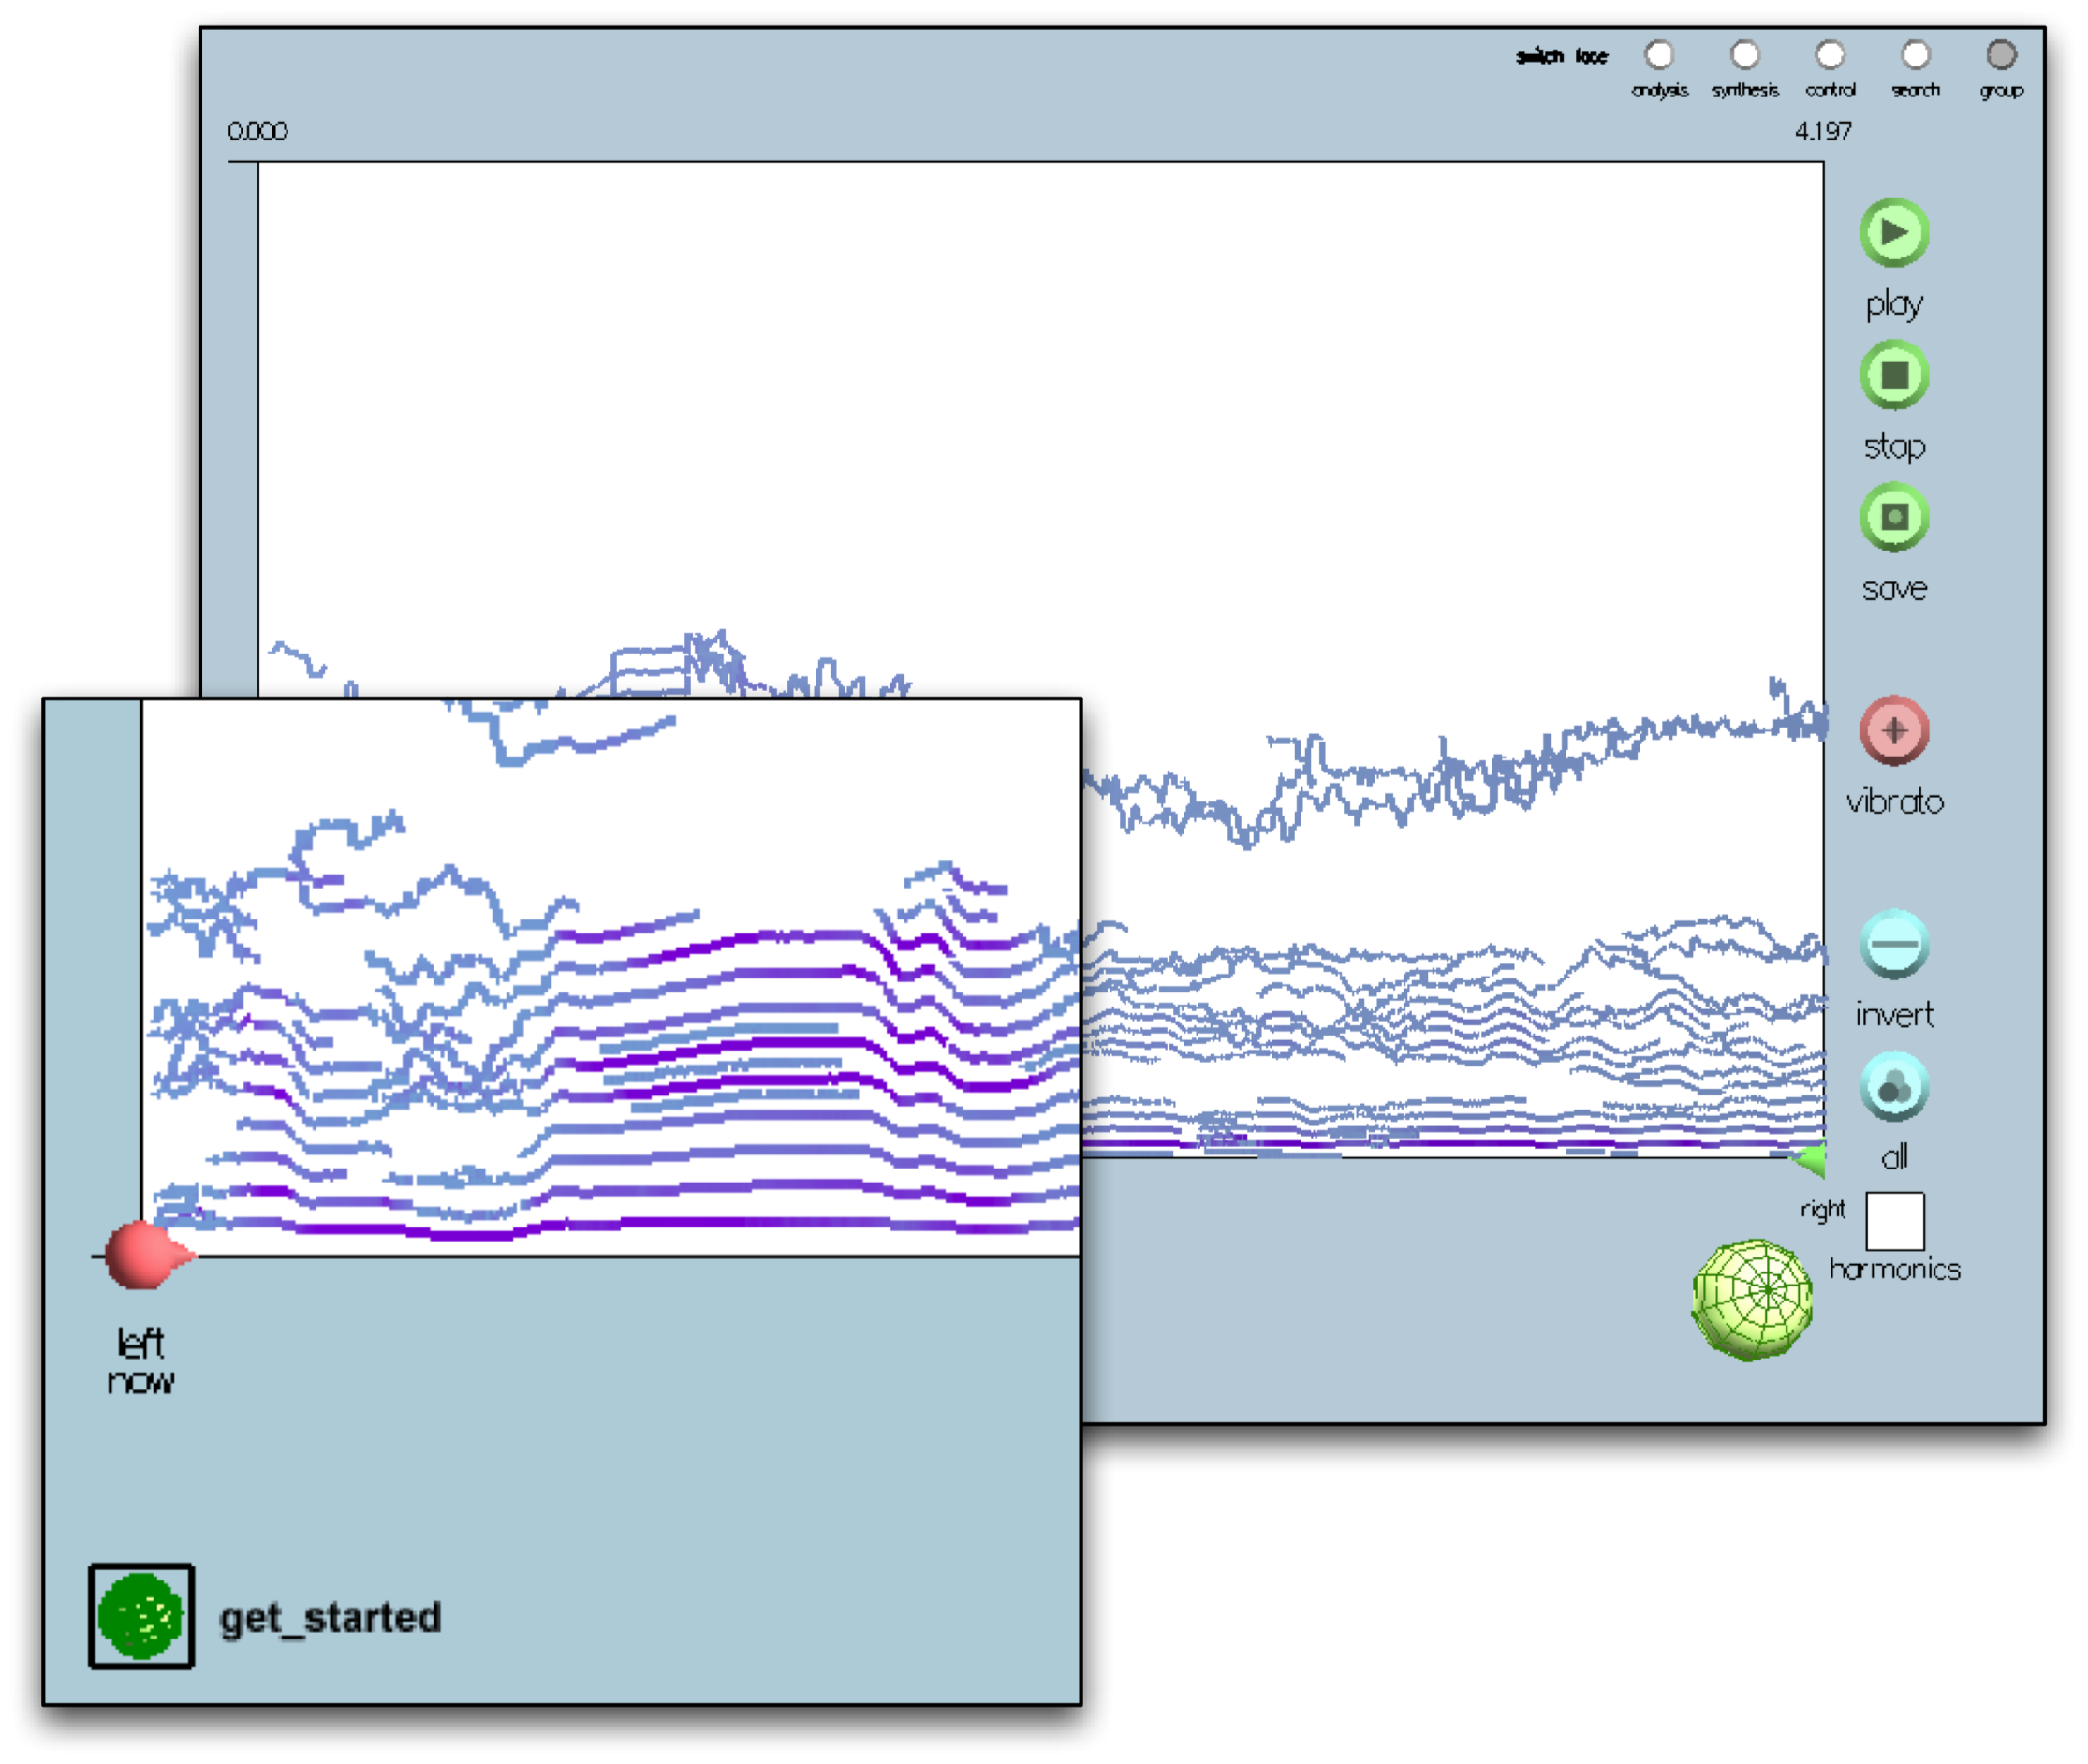
\includegraphics[scale=0.09]{images/group-focused}

\caption{\label{fig:spectrogram}Spectrogram from the analysis face of
TAPESTREA.  The sound is a shooting firework with an explosion at the end. Four
of the harmonic tracks associated with the firecrack's whistling sound have
been marked in bold.}
\end{figure}

TAPESTREA uses a Fast Fourier Transform (FFT) algorithm over a sliding window
to determine the strength of a wide range of frequencies, then graphs it for
the user in the form of a spectrogram on the analysis face.

\begin{figure}
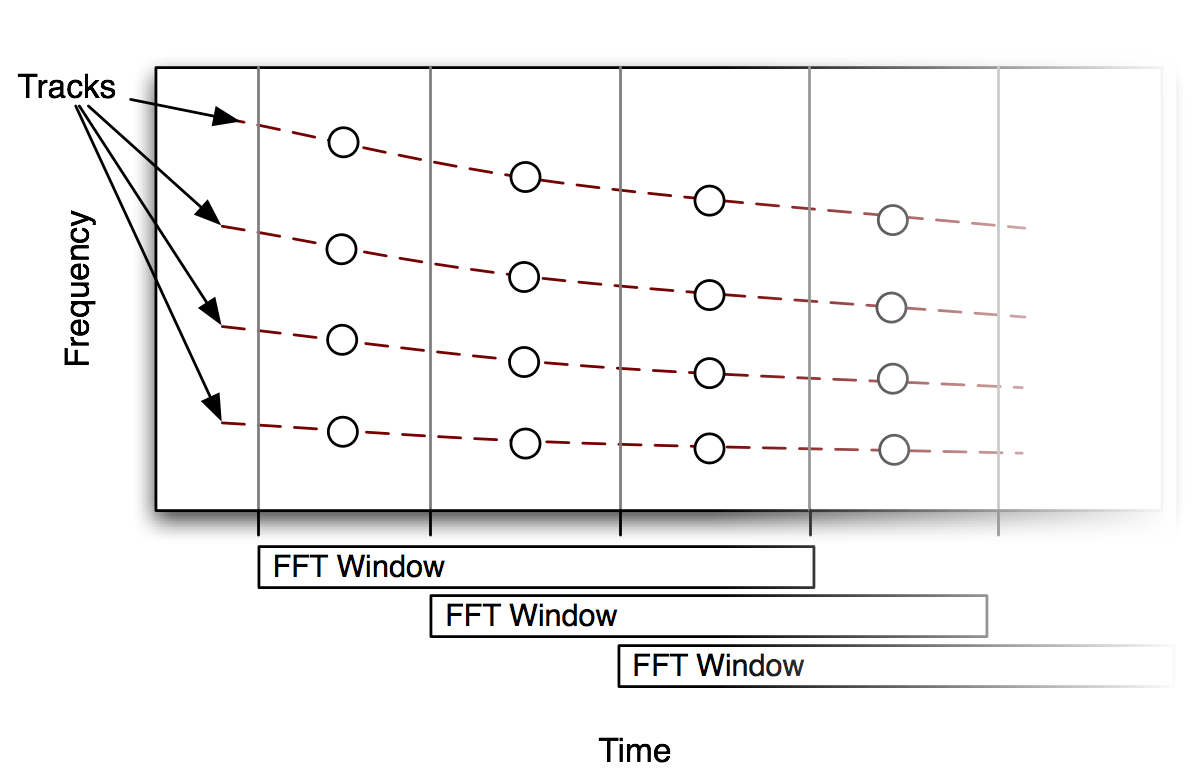
\includegraphics[scale=0.5]{images/trackdots}

\caption{\label{fig:trackdots}Adjacent frequency peaks are connected to create
tracks.}
\end{figure}

A human looking at a graph like that in Figure \ref{fig:spectrogram} can see
that there are several discrete sounds occurring at the same time on the left;
the roughly horizontal, evenly-spaced ``lines'' are the harmonic tones of the
whistling of a firecracker.  A human can think of these as discrete tones, and
so can TAPESTREA by representing them as tracks. The tracks are extracted
according to parameters entered on the analysis face, the most important of
which is the number of tracks to detect. At each of the stopping points of the
sliding FFT window, that number of frequency peaks with the highest magnitude
are stored. They are then matched with similarly detected peaks from adjacent
frames based on an algorithm like nearest neighbor. There are rules for
determining whether a peak is the start of a track, when a track may die, and
so on \cite{recompose}. The end result (see Figure \ref{fig:trackdots}) is that
the tracks that have been created to represent the sinusoidal audio can be used
to approximately recreate the original sound without the other noise.  More
importantly to this paper, tracks are a convenient representation for the
user to interact with in TAPESTREA, as will be shown.

\subsection{Track Internal Representation}

Tracks do not stand on their own in TAPESTREA. \noun{Track} objects are
contained within objects of the \noun{Deterministic} class, which is a
sub-class of \noun{Template} \footnote{\noun{Deterministic} and \noun{Template}
are actually C++ struct types, but they can be thought of as classes for the
purposes of this paper.}.

Templates have a few parameters like gain, pan, and time stretch which are
mapped to controls on the synthesis face. This information can be changed
without modifying the original underlying representation of the audio in the
template. In the case of sinusoidal audio in the \noun{Deterministic}
sub-class, the underlying representation is a set of tracks.

\begin{figure}
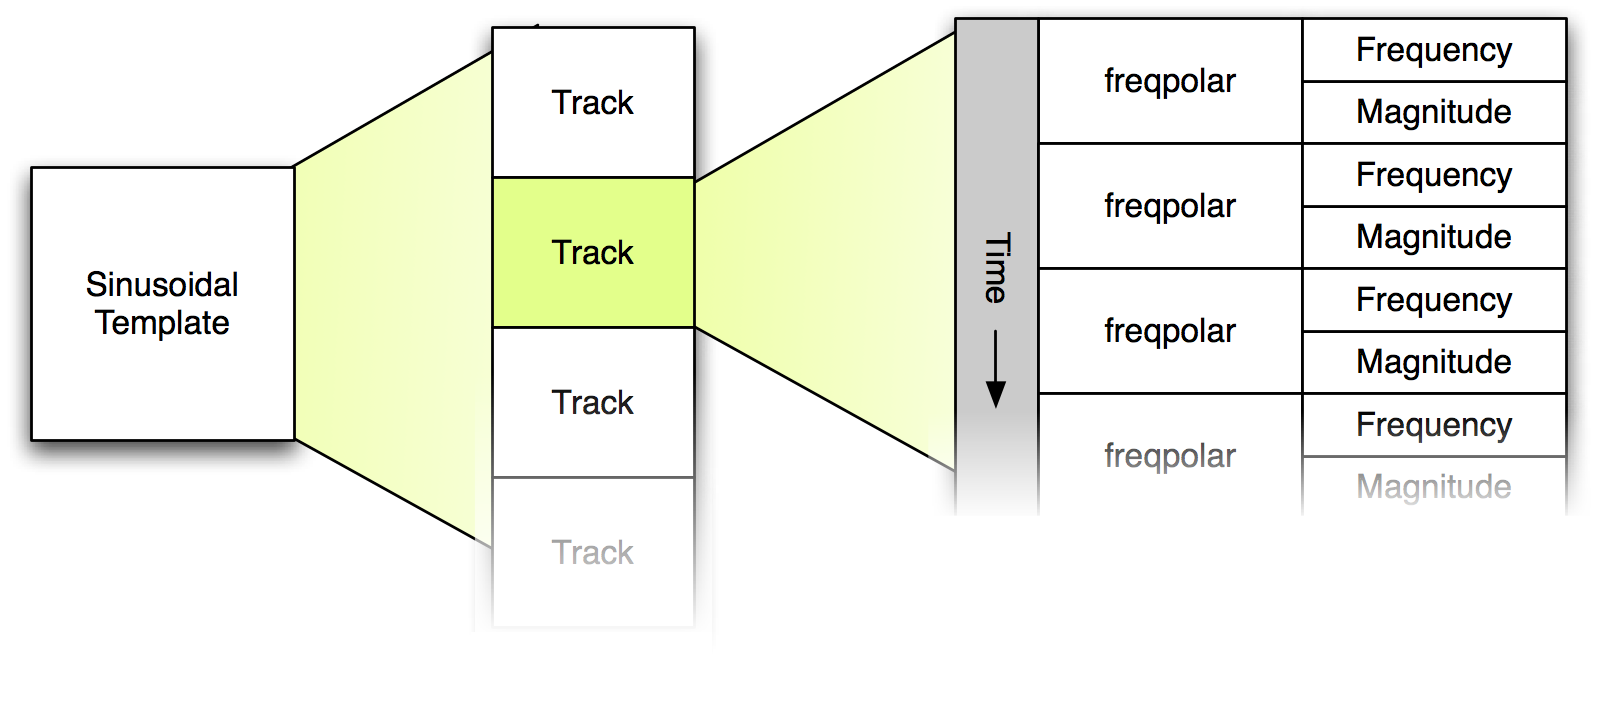
\includegraphics[scale=0.4]{images/deterministic}

\caption{\label{fig:sinusoidal}A sinusoidal template is a container for one or
more tracks. The tracks each contain an array of `freqpolar' objects with
frequency and magnitude values.}
\end{figure}

Tracks have a small bit of data about their start time, end time, and phase,
but most importantly they have an array of \noun{freqpolar} objects. The
\noun{freqpolar} objects are used for storing the frequency, the time at which
it was detected, and the magnitude of the frequency peak.

\subsection{Tracks to the User -- The Group Face}

The added functionality in VTAPS for track-based editing is on the ``group''
face, a screenshot of which is in Figure \ref{fig:group-face}. The group face
consists of a display similar to a spectrogram, a library of available
templates, buttons to control playback, a button to add vibrato, a button to
invert the track selection, a checkbox to control whether harmonic tracks are
selected when a track is clicked, and buttons for other added features.

\begin{figure}
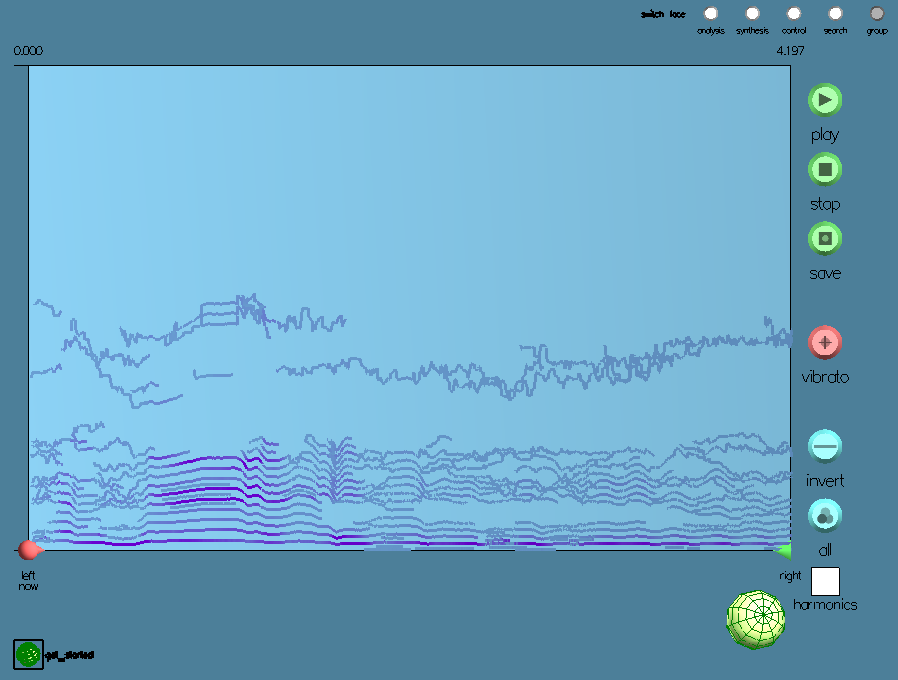
\includegraphics[scale=0.25]{images/group}

\caption{\label{fig:group-face}Screenshot of the ``group'' face}
\end{figure}

\subsubsection{The Group Face Spectrogram}

The analysis face has a spectrogram that reflects the strength of all
frequencies in the scanning range in the color that is drawn. The spectrogram
on the group face does the same thing for only the frequencies and times that
are present in the currently displayed tracks. The detected peaks at each time
are colored according to their strength, but other frequencies are not colored
at all.

This spectrogram is also different in that it allows the individual tracks to
be selected or deselected with the mouse by clicking. Only tracks that have
been selected will be played back (the others are colored white), so
``what-if'' experiments can be quickly performed by clicking tracks and
templates.

There are also buttons for inverting the current selection (deselecting
selected tracks and vice-versa) and selecting all tracks.

\subsubsection{The Template Library}

Unlike in other faces, the template library on the group face only shows
sinusoidal templates, because those are the only templates with tracks. Also
unique to this face is the ability for multiple templates to be selected at one
time. When a template it selected, its tracks are added to the spectrogram, and
are removed when the track is deselected.

When the save button is pressed, currently selected tracks are saved to a new
sinusoidal template regardless of which template they were originally a part
of. The new template can be modified without disturbing the originals.

\subsubsection{Vibrato}

The ``vibrato'' button adds a vibrato to selected tracks.The vibrato effect is
added by iterating over each of the selected track's \noun{freqpolar} objects
and multiplying the frequency by $1+\alpha\sin(2 \pi f_v t)+\beta*r$, where
$\alpha$ is the amount of periodic vibrato, $f_v$ is the vibrato frequency,
$\beta$ is the amount of random vibrato, and $r$ is a random sequence whose
parameters can be set by the user.  The vibrato of all tracks will be
synchronized.


\subsubsection{\label{sub:harmonic-selection}Harmonic Selection}

The checkbox labeled ``harmonics'' enhances track selections by also applying
the selection to tracks that appear to be harmonics (multiples) of the one that
was clicked. Clicking a deselected track will select that track as well as any
tracks that, at the time along the axis at which you clicked, also have a
frequency within a small percentage of an integer multiple of the original
track's frequency.

By only considering each track's frequency at that time, the user is given the
ability to select tracks which are harmonic at one point even if they are are
not harmonic at others. This is convenient because of errors in detecting
tracks that cause non-pitched sounds to be merged into tracks in the form of
random-seeming modulation. If the whole track were considered, this noise would
cause some harmonic tracks to be left undetected.

% Even/odd?

\section{Applications and Examples}

What follows are in-depth descriptions of a few of the techniques enabled by
the addition of VTAPS.

\subsection{Arbitrary Filtering}

One obvious application of the group face is the filtering of high or low
frequencies of a piece of audio. This is easily done by removing the tracks
above (low-pass) or below (high-pass) a certain frequency.  This is more
stringent than actual high- and low-pass filters, that only reduce the
amplitude of filtered frequencies, not always eliminating them \cite[pg
29-31]{real}. The effect of a traditional filter can be emulated by reducing the 
gain on the high- and low-frequency tracks. Since track synthesis in TAPESTREA 
is accomplished by additive sinusoids, any filtering, no matter how extreme, is 
guaranteed not to cause aliasing. 
%components. 
%saving the
%high frequencies and the low frequencies as templates, then recombining them
%with different gains on the synthesis face \footnote{This is a tedious process
%that would be made easier by improvements descripted in Section
%\ref{sec:Future-Work}.}.

\subsection{Clean Extraction}

%The salient frequencies of sinusoidal audio are recognized by the peaks in a
%spectrogram representation of the sound. These frequencies do not necessarily
%equate to tracks detected by TAPESTREA, however, due to the problem of wedging.

The method of extracting tracks from audio by block selection on the
spectrogram has a problem dealing with unwanted tracks. These are
tracks which intersect the smallest rectangle one can draw to encompass the
tracks one actually wants. Decreasing the number of tracks to detect solves
this problem for low-power unwanted tracks, but high-power tracks that are more
prominent than the wanted tracks will be extracted in their stead.

The group face is useful for solving this problem. 
%with only slight tedium. 
One can set the number of tracks to detect (the number of simultaneous tracks
allowed at any point in time) to the number of wanted tracks plus some extra tracks. 
%the number of wedged tracks. 
The unwanted tracks can then be removed by clicking them, leaving
only the wanted tracks.

\subsection{Time, Amplitude, and Frequency Manipulations}

The ability to recombine tracks gives way naturally to the desire to adjust them
to mix together better. Shifting individual tracks in time allows one to rearrange 
a template and to flexibly combine selected tracks from different parts of different 
templates. Similarly, it is useful to adjust the amplitude of tracks 
at various points to emphasize certain frequencies or make others stand out less. 
A track or set of tracks can also be individually time-stretched or shifted in frequency.

Other frequency manipulations on individual tracks include quantizing 
the frequencies to a fixed scale for interesting vocal effects. Another possibility 
to explore is the smoothing of a track's frequency trajectory by matching it to a spline 
or processing it with a low-pass filter. 
 
%Currently, templates are assumed to start exactly when
%the first track begins to play, which hinders attempts to combine tracks from
%two clips that are not meant to start at the same time. Similarly, it would be
%useful to be able to adjust the amplitude of tracks at various points to
%emphasize certain frequencies or make others stand out less.
%\subsection{Frequency Transposition}
%The method for increasing pitch as described in Section
%\ref{sub:pitch-shifting} is crude in that pitch can only be changed an octave
%at a time. It would be useful to be able to transpose by any amount by
%multiplying a selected track's frequencies by some constant.

\subsection{Track Slicing}

The track extraction algorithms are at most as perfect as the user, so there
are times when a track jumps from one perceived frequency peak to another that
is inconvenient or unnatural for the user to work with -- for example, a track
that jumps from one harmonic to the next is inconvenient, but happens when they
are spaced closely.  Hence, it is helpful for a user to be able to split this track into two by
selecting the time at which they are perceptually discontinuous.

\subsection{\label{sub:pitch-shifting}Working with Harmonics}

VTAPS includes the option to select the harmonics of a given track. These 
harmonics can then be treated as a group for special processing. 

For example, the pitch of harmonic sounds can be shifted up by one octave by deleting the
even harmonic frequencies. While all harmonics are selected by checking the
``harmonics'' checkbox and clicking on the first harmonic track, clicking the
second harmonic track deselects all of the even harmonics, bumping the
pitch by one octave.
The odd harmonics can be selected by pressing the ``invert'' button after the
even harmonics have been selected.

The ability to select even and odd harmonics allows the user to apply different 
effects to different harmonic groups within a template. Thus, odd and  even harmonics 
can have different vibrato, as well as amplitude, time, and frequency transformations, 
for instance to create the effect of two singers doubling each other at an octave. 
Another use for track-specific manipulations within a template is to  
facilitate transforming only the vowel sounds (typically having harmonics), leaving 
consonants intact. 

%\subsection{Harmonic Detection and Manipulation}
%
%There is a check box called ``group'' on the analysis face of TAPESTREA that
%was present before VTAPS. When checked before the ``separate'' button is
%pressed to extract components from a loaded audio piece, the sinusoidal
%components are automatically grouped by matching harmonicity, modulation, and
%start and end times \cite{recompose}.  These groups can be saved to separate
%templates.
%
%Selecting tracks on the group face with the ``harmonics'' check box selected
%can be similarly used to create templates containing only a set of harmonic
%tracks, although as explained in Section \ref{sub:harmonic-selection}, the
%criteria is more loose. Onset and offset times, and modulation are not taken
%into account, which can be good or bad depending on the desired result.


\section{\label{sec:Future-Work}Future Work}
% Do some of these and move to section 3

While VTAPS offers interactive track-level manipulation to modify templates in 
new ways, there is plenty of scope for future expansion. The ability to cut, paste, 
replicate and move selections of tracks together would be a useful advantage. 
Another desirable feature is the capability to add sub-harmonics to a template. 
These would be a new set of harmonics based on a fundamental at an integer 
division of the existing fundamental, usually at a lower amplitude than the main 
harmonics. Adding subharmonics could give a sense of roughness to the voice, 
as is often heard in Blues singers. 

Another avenue to explore is the identification of formants from a set of tracks. 
When altering the frequency of vocal sounds, the vowels often change as well. 
Analyzing selected tracks to locate the formants of the vowel sounds could lead 
to intelligent frequency transformations that leave the vowels relatively unchanged. 

\section{Conclusions}

Previously, the only power the user had over the tracks in a sinusoidal
template was to adjust parameters on the analysis face to control the tracks'
extraction, and to adjust parameters like gain and pitch on the synthesis face.
With the group face, users can edit a template without extracting again, and do
so even after the source audio is long gone.

The group face provides instant gratification in the sense that experimenting
with the inclusion or removal of tracks of a certain frequency can now be done
in seconds and with a few clicks. It benefits sound producers who wish to
exercise more full control over what frequencies go into the final piece, and
audio enthusiasts with a more educational mindset who simply want to understand
how audio signals work.

%There are many ideas of what lies behind the doors the group face has opened,
%and its development is only just beginning.

\begin{thebibliography}{citations}

\bibitem{clam} Amatriain, X. and P. Arumi. ``Developing Cross-platform Audio and Music 
Applications with the CLAM Framework'', {\it Proc. ICMC}, Barcelona, Spain, 2005. 
%{\it Proceedings of the International Computer Music Conference}

\bibitem{audiosculpt} Bogaards, N., A. Robel, and X. Rodet. ``Sound Analysis and Processing 
with AudioSculpt 2'', {\it Proc. ICMC}, Miami, USA, 2004. 

\bibitem{real} Cook, P. R. {\it Real Sound Synthesis for Interactive
Applications}. A. K. Peters, Natick, Massachusetts, 2002.

\bibitem{lemur} Fitz, K. and L. Haken. ``Sinusoidal Modeling and Manipulation Using Lemur'', 
{\it Computer Music Journal 20:4}, 1996. 

\bibitem{spear} Klingbeil, M. ``Software for Spectral Analysis, Editing, 
and Synthesis'', {\it Proc. ICMC}, 
Barcelona, Spain, 2005. 

\bibitem{mq} McAulay, R. J. and T. F. Quatieri. ``Speech Analysis / Synthesis Based on a 
Sinusoidal Representation'', {\it IEEE Transactions on Acoustics, Speech, and Signal Processing 34:4}, 1986.

\bibitem{recompose} Misra, A., P. R. Cook, and G. Wang. ``Musical
Tapestry: Re-Composing Natural Sounds'', {\it Proc. ICMC}, New Orleans, USA, 2006.

%\bibitem{paradigm} Misra, A., P. R. Cook, and G. Wang. ``A New Paradigm
%for Sound Design'', {\it Proceedings of the 2006 International
%Conference on Digital Audio Effects (DAFx)}, Montreal, Canada, 
%2006.

\bibitem{chuck} Wang, G. and P. R. Cook. ``ChucK: A Concurrent, On-the-fly, Audio Programming 
Language'', {\it Proc. ICMC}, Singapore, 2003.

\bibitem{sms} Xerra, S. {\it A System for Sound Analysis / Transformation / Synthesis based on a 
Deterministic plus Stochastic Decomposition}. Ph.D. thesis, Stanford University, 1989. 


\end{thebibliography}

\end{document}
